\documentclass[12pt]{report}

\usepackage{graphicx}
\graphicspath{ {./images} }

\usepackage{parskip}
\setlength{\parskip}{\baselineskip}
\setlength{\parindent}{0pt}

\title{Jane Goodall Script}
\author{Rayhan \and Odi \and Bagas}

\begin{document}

\maketitle

\centering

\section*{Orientation of Jane Goodall}

Meet Jane Goodall, one of the pioneering English primatologists. Goodall is
well known for her expansive research and dedication in order to save the lives
of chimpanzees around the world.

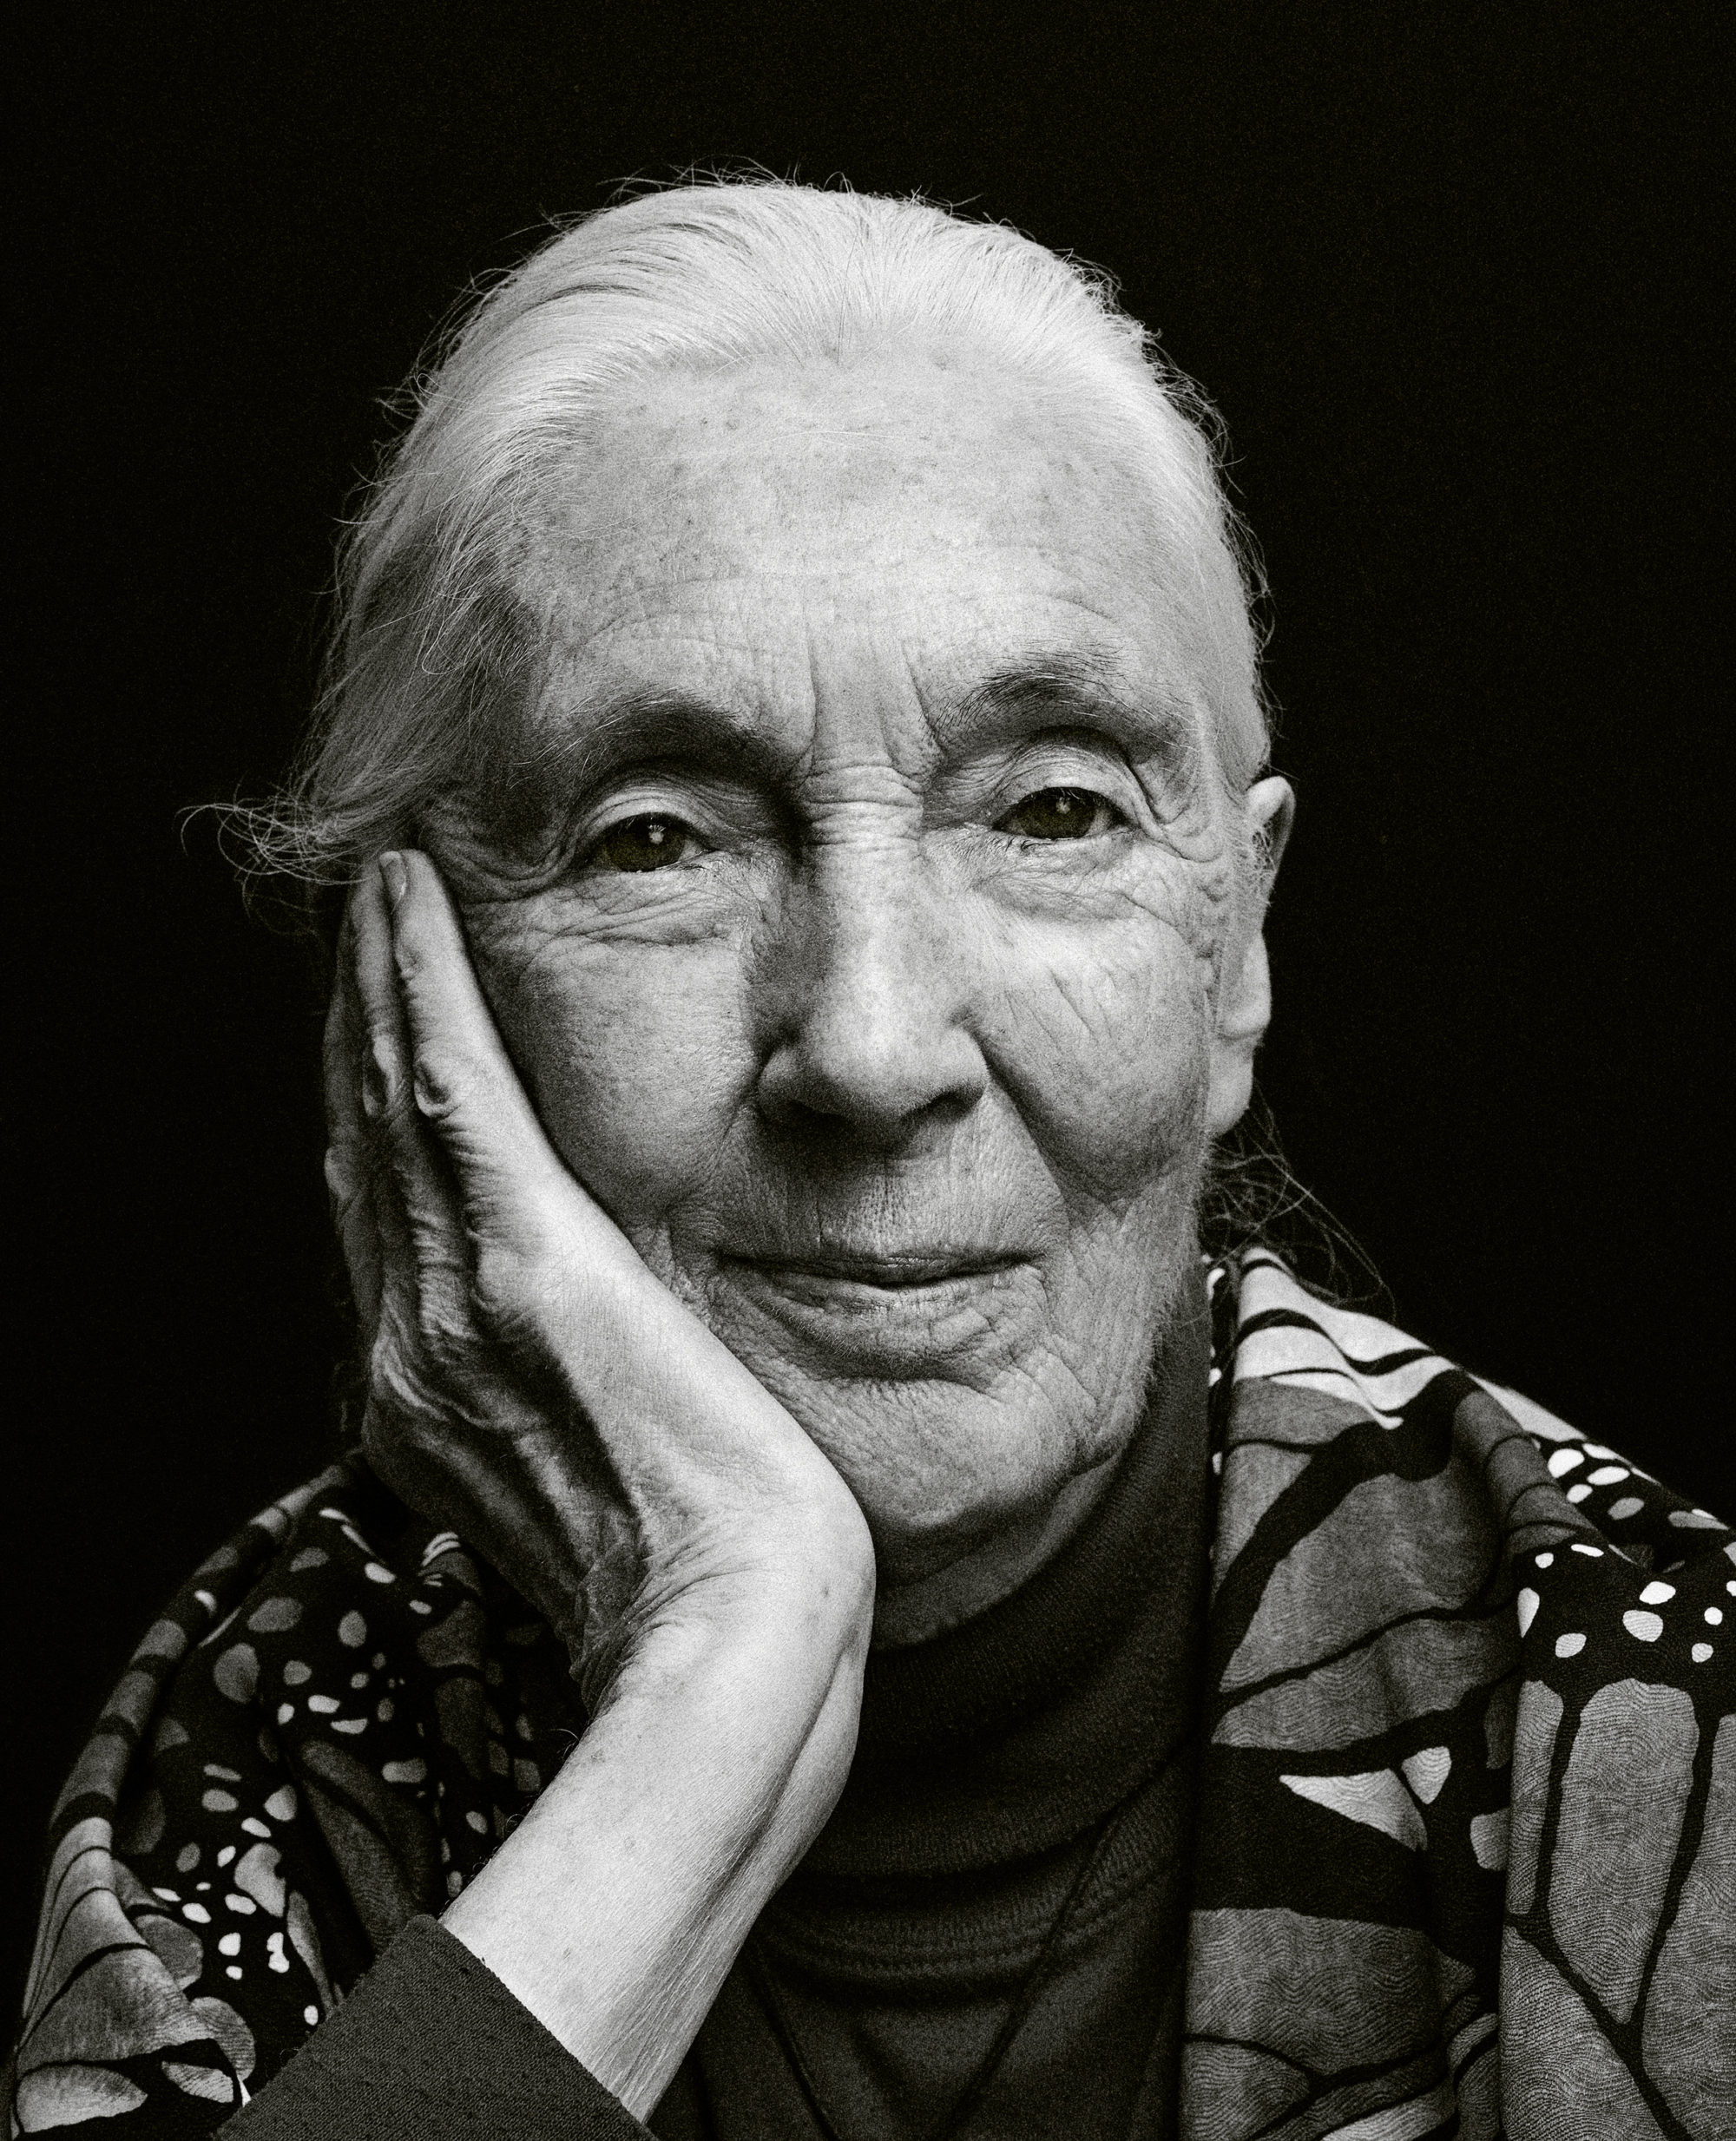
\includegraphics[
    width=7cm,
    height=10cm,
    keepaspectratio
]{jane-goodall-introduction}

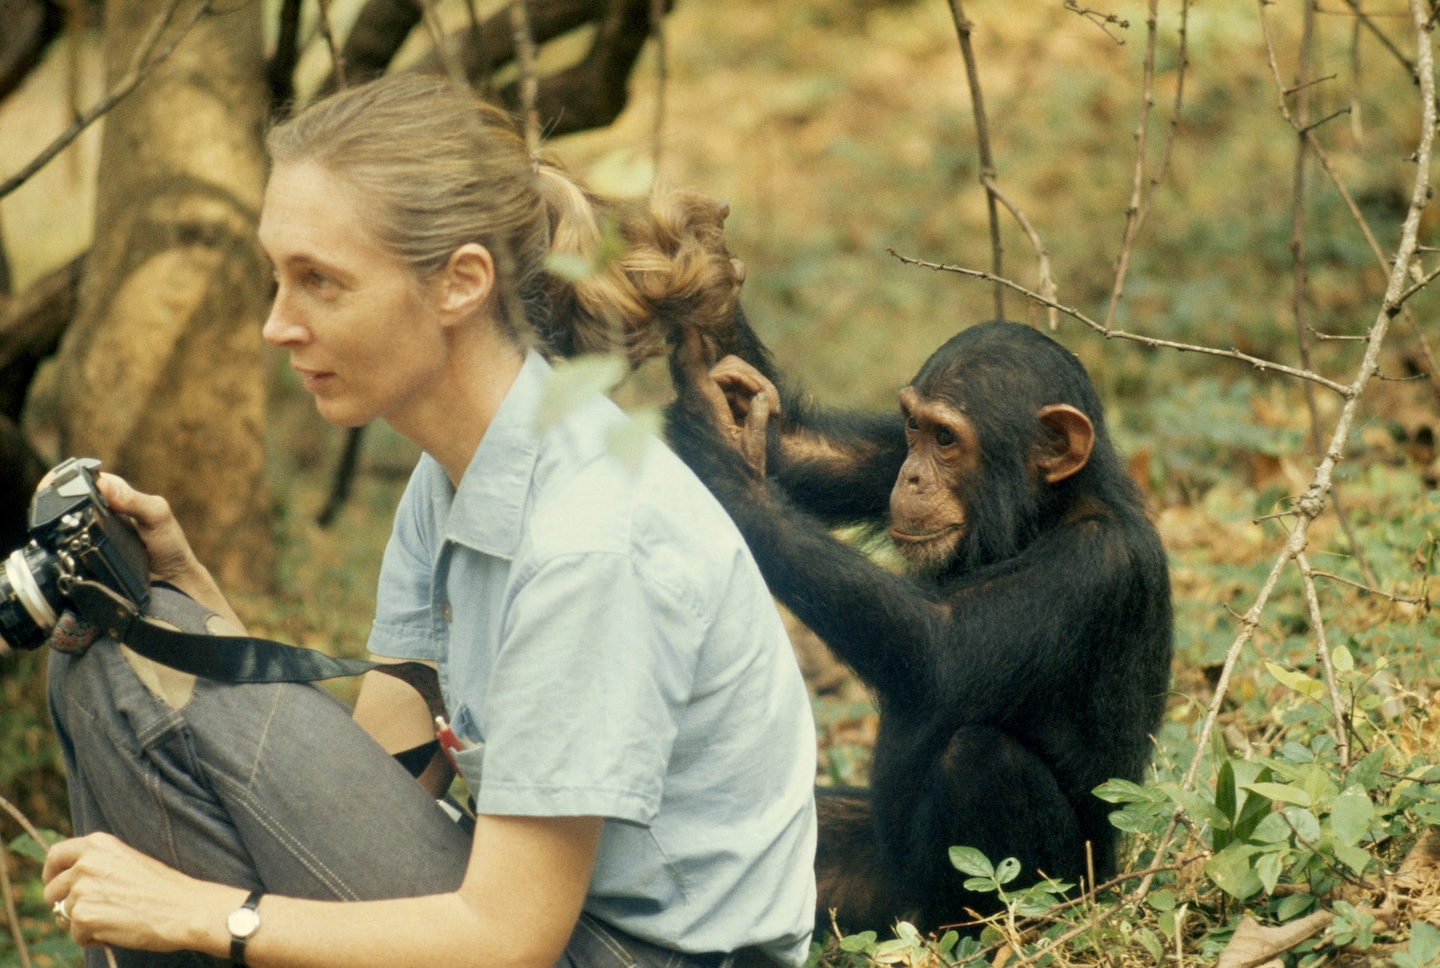
\includegraphics[
    width=10cm,
    height=20cm,
    keepaspectratio
]{jane-goodall-introduction-2}

\pagebreak

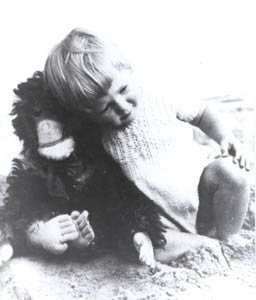
\includegraphics[
    width=6cm,
    height=15cm,
    keepaspectratio
]{jane-goodall-jubilee}

Her sheer passion was all thanks to Jubilee, a chimpanzee doll Goodall acquired
during her first birthday. This was what sparked Goodall's unadulterated
fascination with chimpanzees.

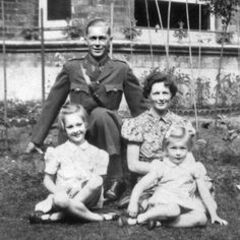
\includegraphics[
    width=6cm,
    height=15cm,
    keepaspectratio
]{jane-goodall-family}

Goodall was the daughter of Margaret Myfanwe Joseph, who worked as a novelist,
and motorsports racer \& businessman Mortimer Morris-Goodall, who was also the
founder of the Aston Martin Owners Club.

\pagebreak

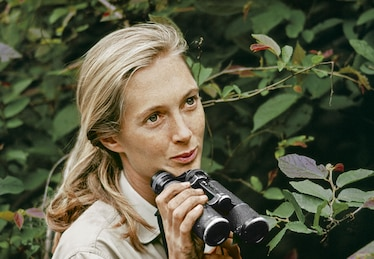
\includegraphics[
    width=8cm,
    height=18cm,
    keepaspectratio
]{jane-goodall-cinematography}

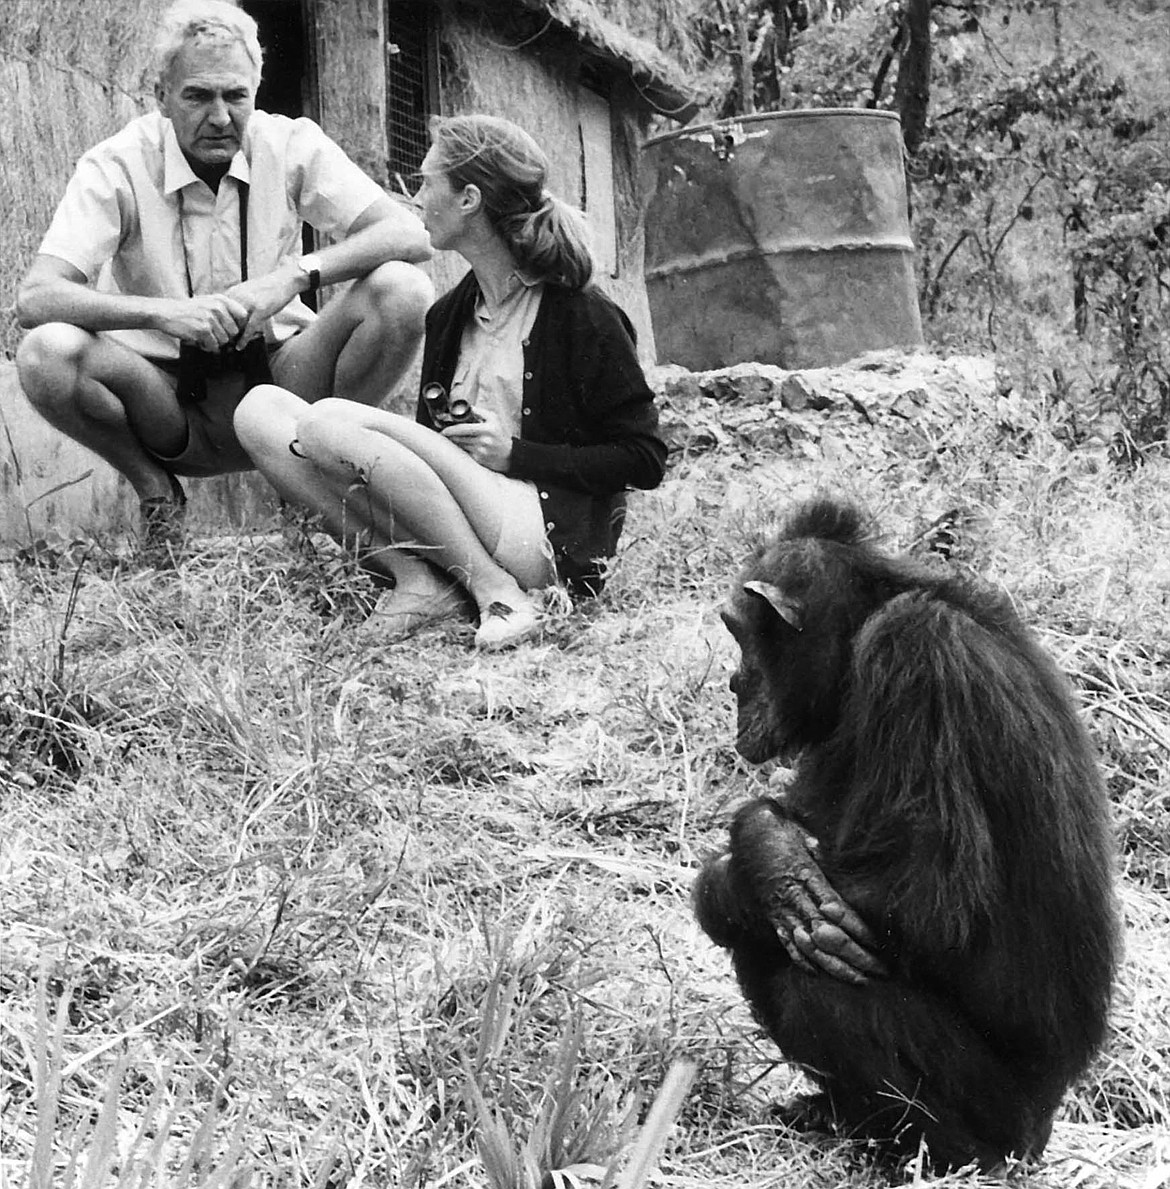
\includegraphics[
    width=8cm,
    height=18cm,
    keepaspectratio
]{jane-goodall-partner}

Aside from an activist, Goodall even worked as a film production assistant and
her own friend's secretary advisor during his research.

\pagebreak

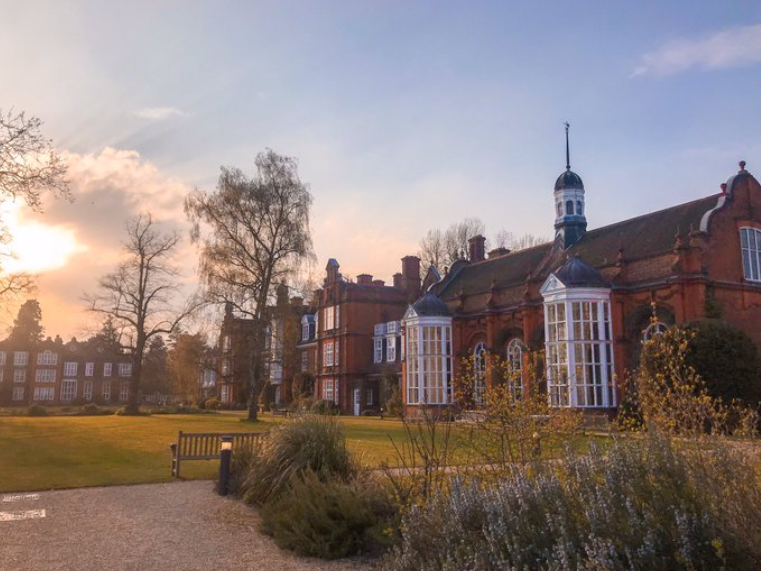
\includegraphics[
    width=10cm,
    height=10cm,
    keepaspectratio
]{newnham-college}

For university, Goodall first went to Newnham College, where she eventually
received her Bachelor of Arts in natural sciences.

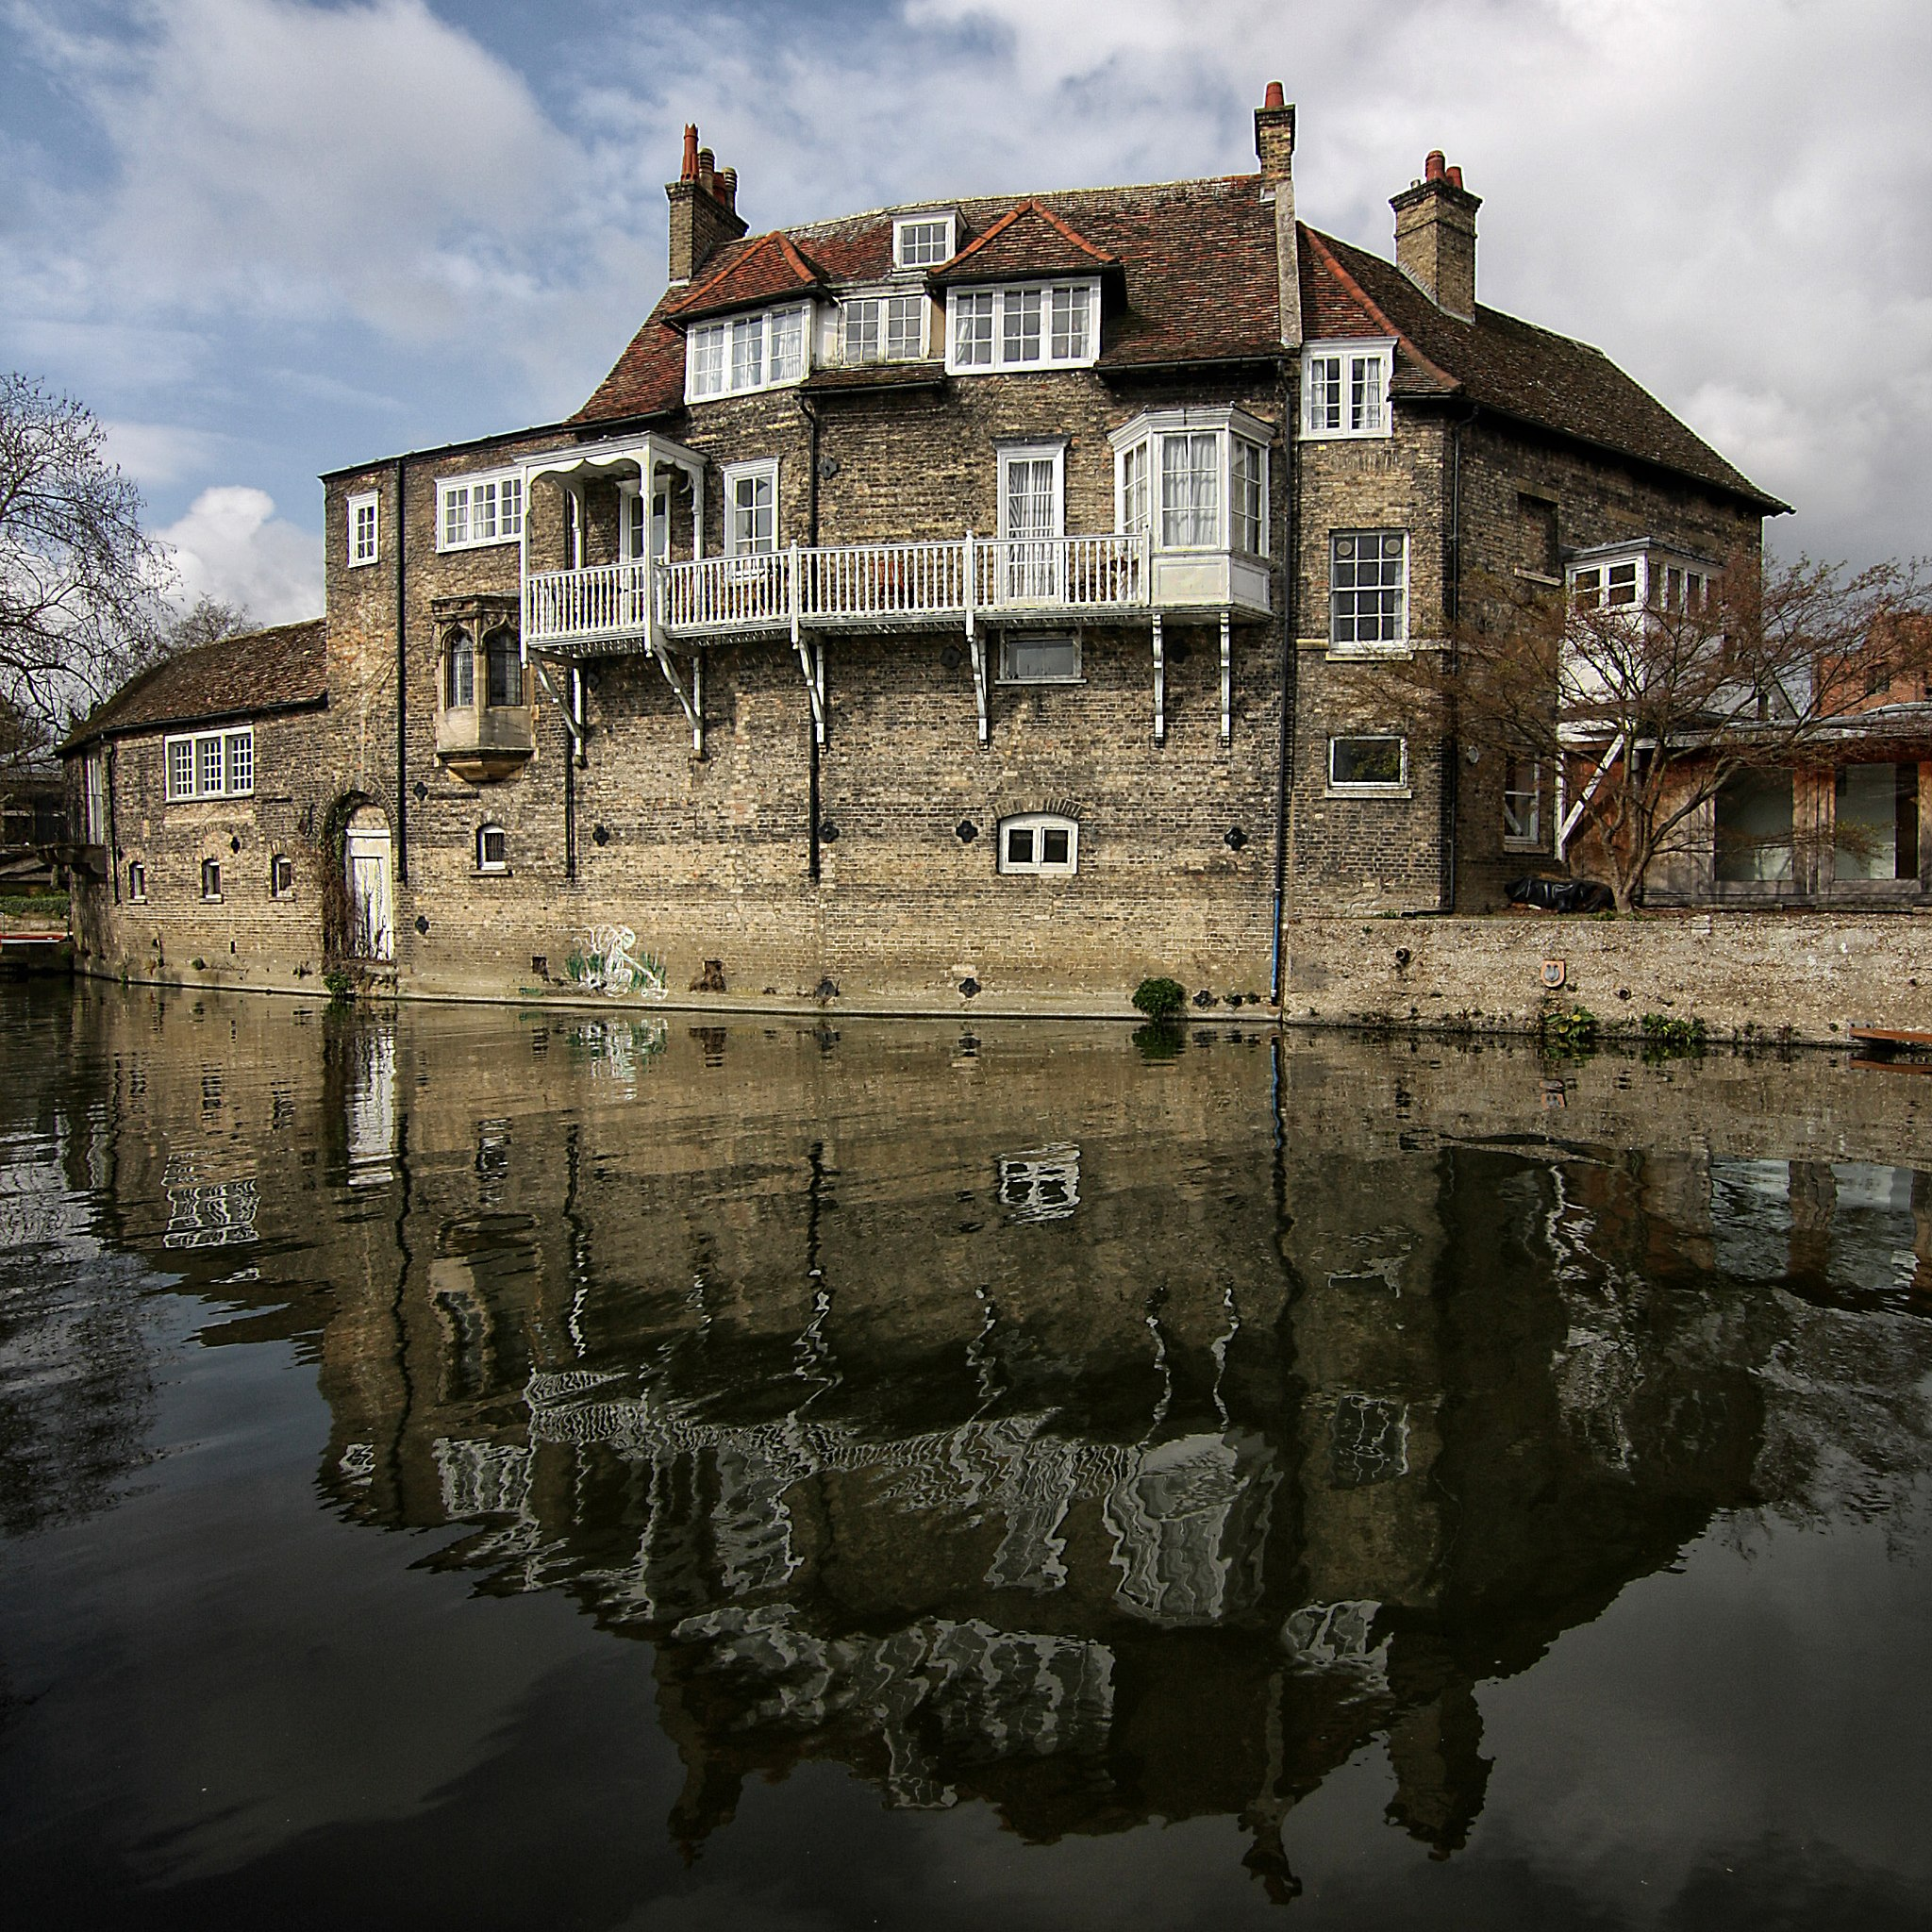
\includegraphics[
    width=8cm,
    height=18cm,
    keepaspectratio
]{darwin-college}

And that is when she attended Darwin College, aiming for a Doctor of Philosophy
in ethology.

\pagebreak

At one point, Goodall was eventually married to Hugo van Lawick from 1964 to
1974 and Derek Bryceson in the year 1975.

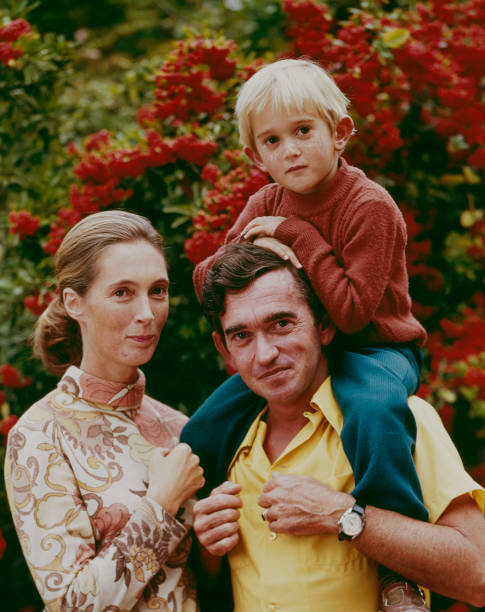
\includegraphics[
    width=7cm,
    height=7cm,
    keepaspectratio
]{jane-goodall-hugo}

Jane Goodall with Hugo Van Lawick

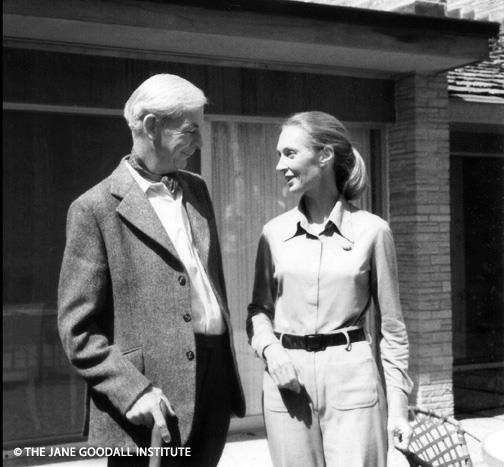
\includegraphics[
    width=8cm,
    height=8cm,
    keepaspectratio
]{jane-goodall-bryceson}

Jane Goodall with Derek Bryceson

\section*{Events of Jane Goodall}

In 1957, Jane Goodall traveled to Kenya to visit his friend family and meet
Louis Leakey, who is a paleontologist and anthropologist.

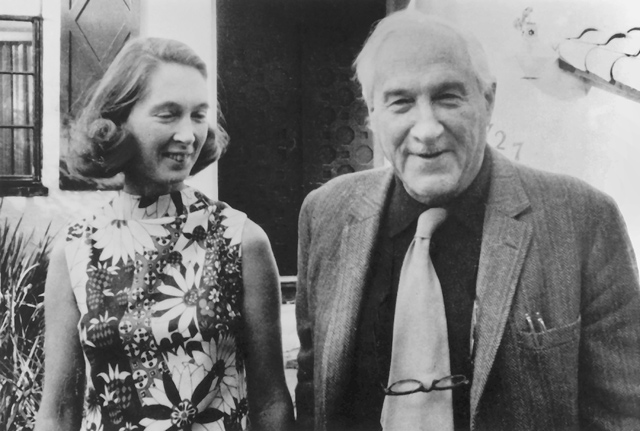
\includegraphics[
    width=10cm,
    height=10cm,
    keepaspectratio
]{jane-goodall-leakey}

During her time in Kenya, she worked as Louis Leaky’s secretary, assisting him
during his research.

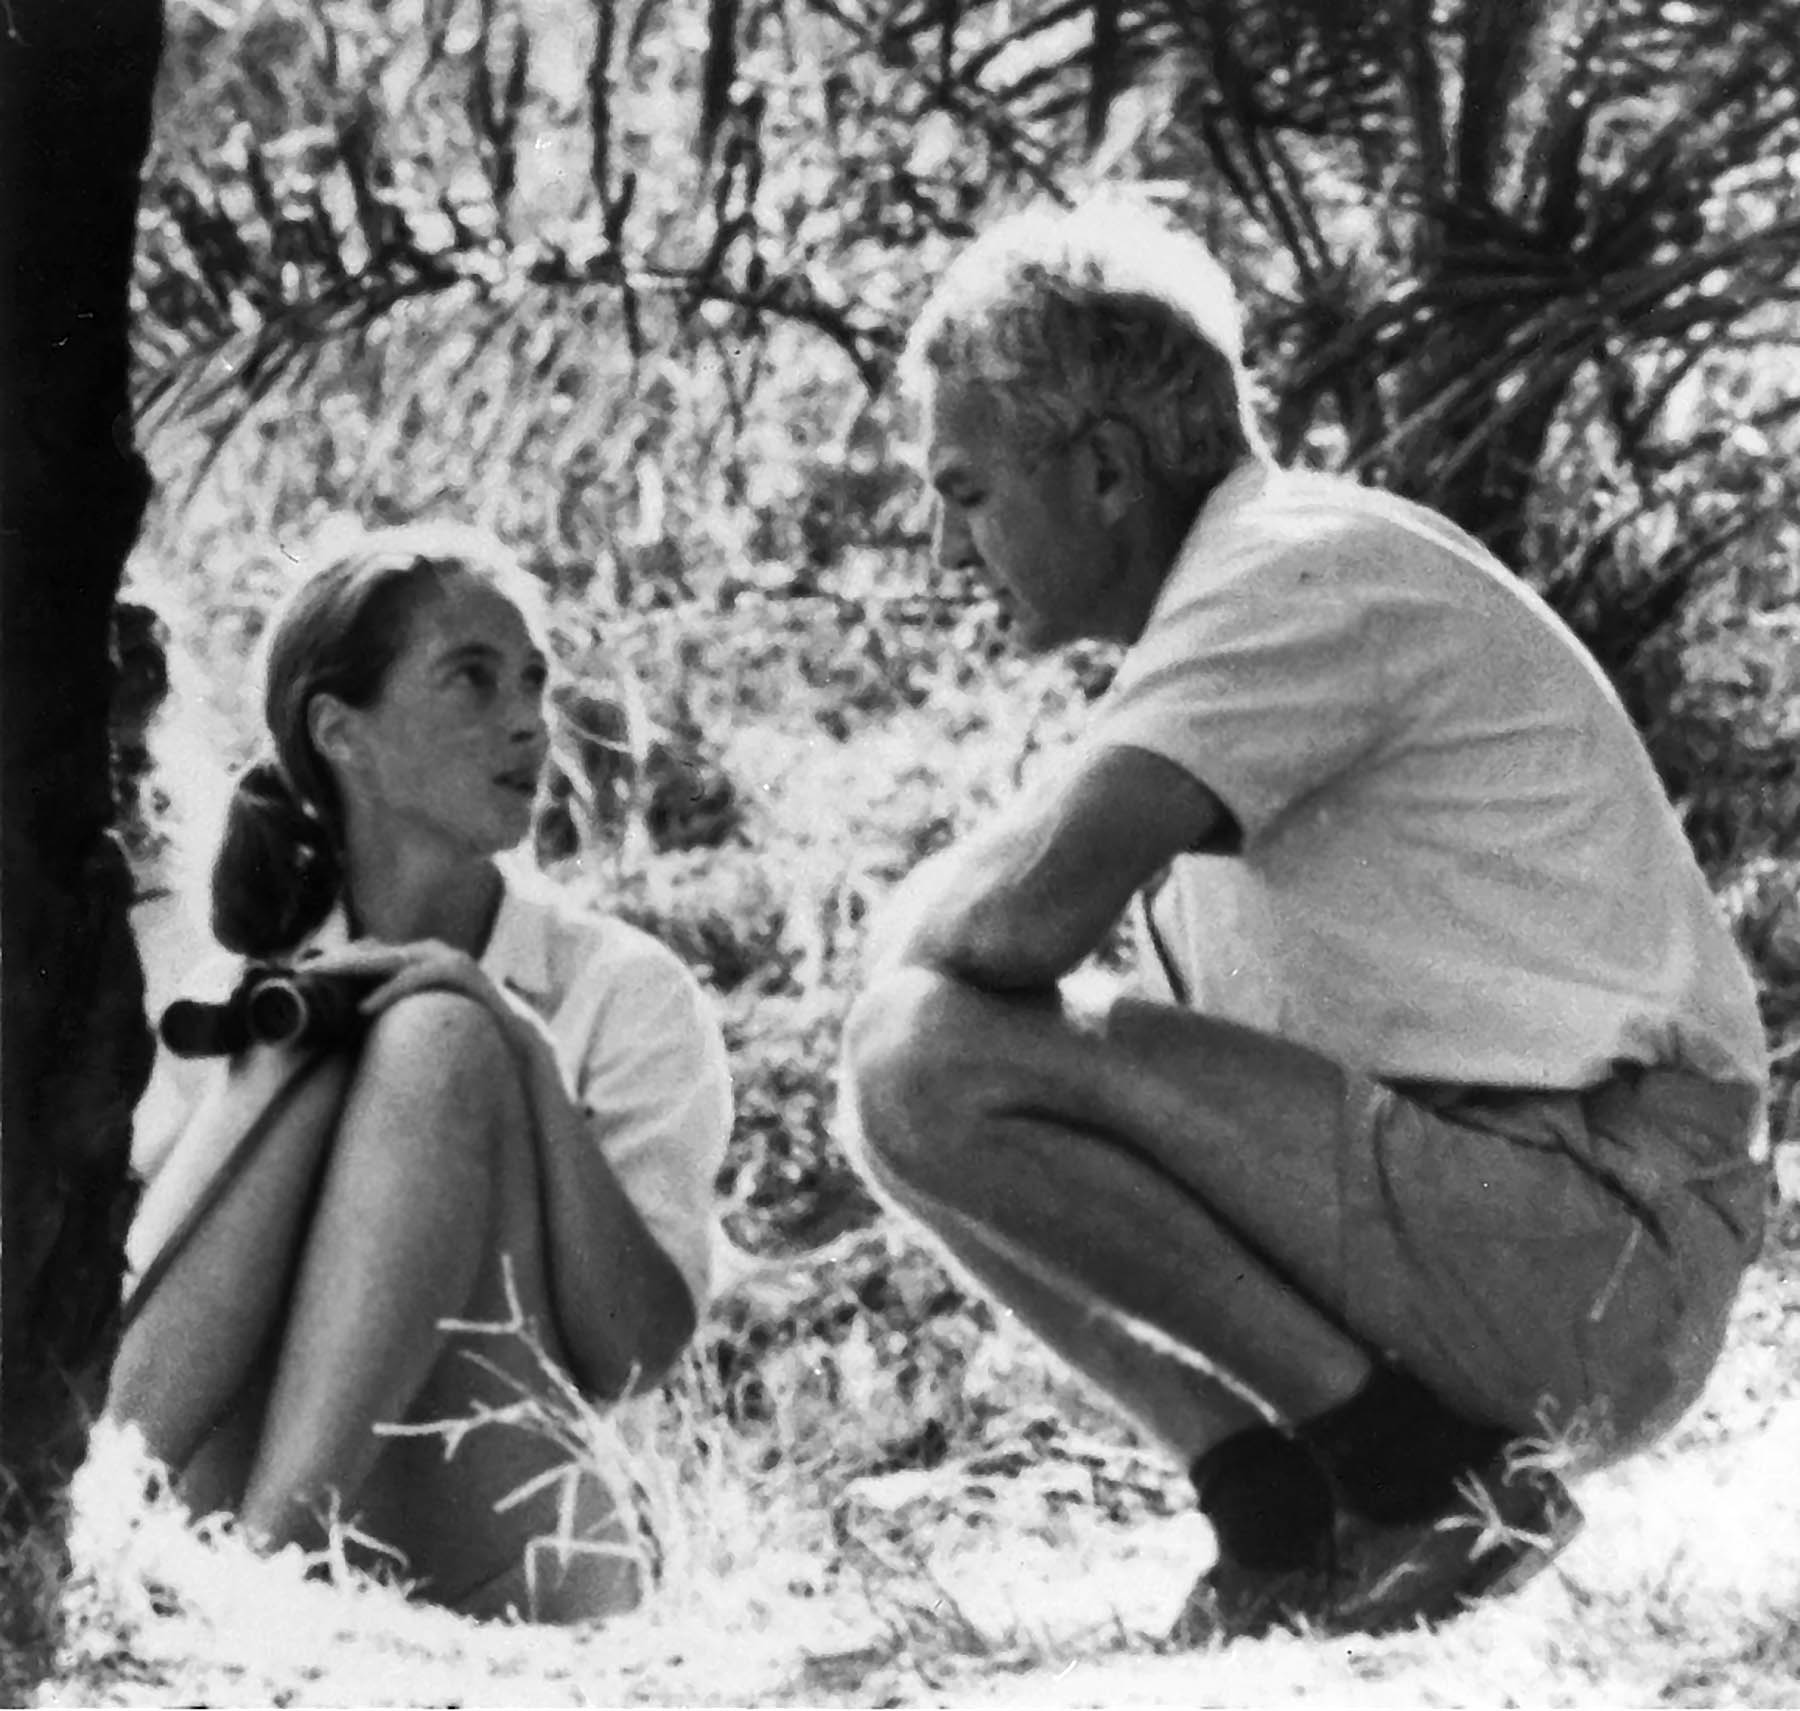
\includegraphics[
    width=8cm,
    height=8cm,
    keepaspectratio
]{jane-goodall-leakey-research}

\pagebreak

3 years later, in 1960, Jane Goodall traveled to Gombe and Tanzania to observe
chimpanzees and their behavior in natural habitat.

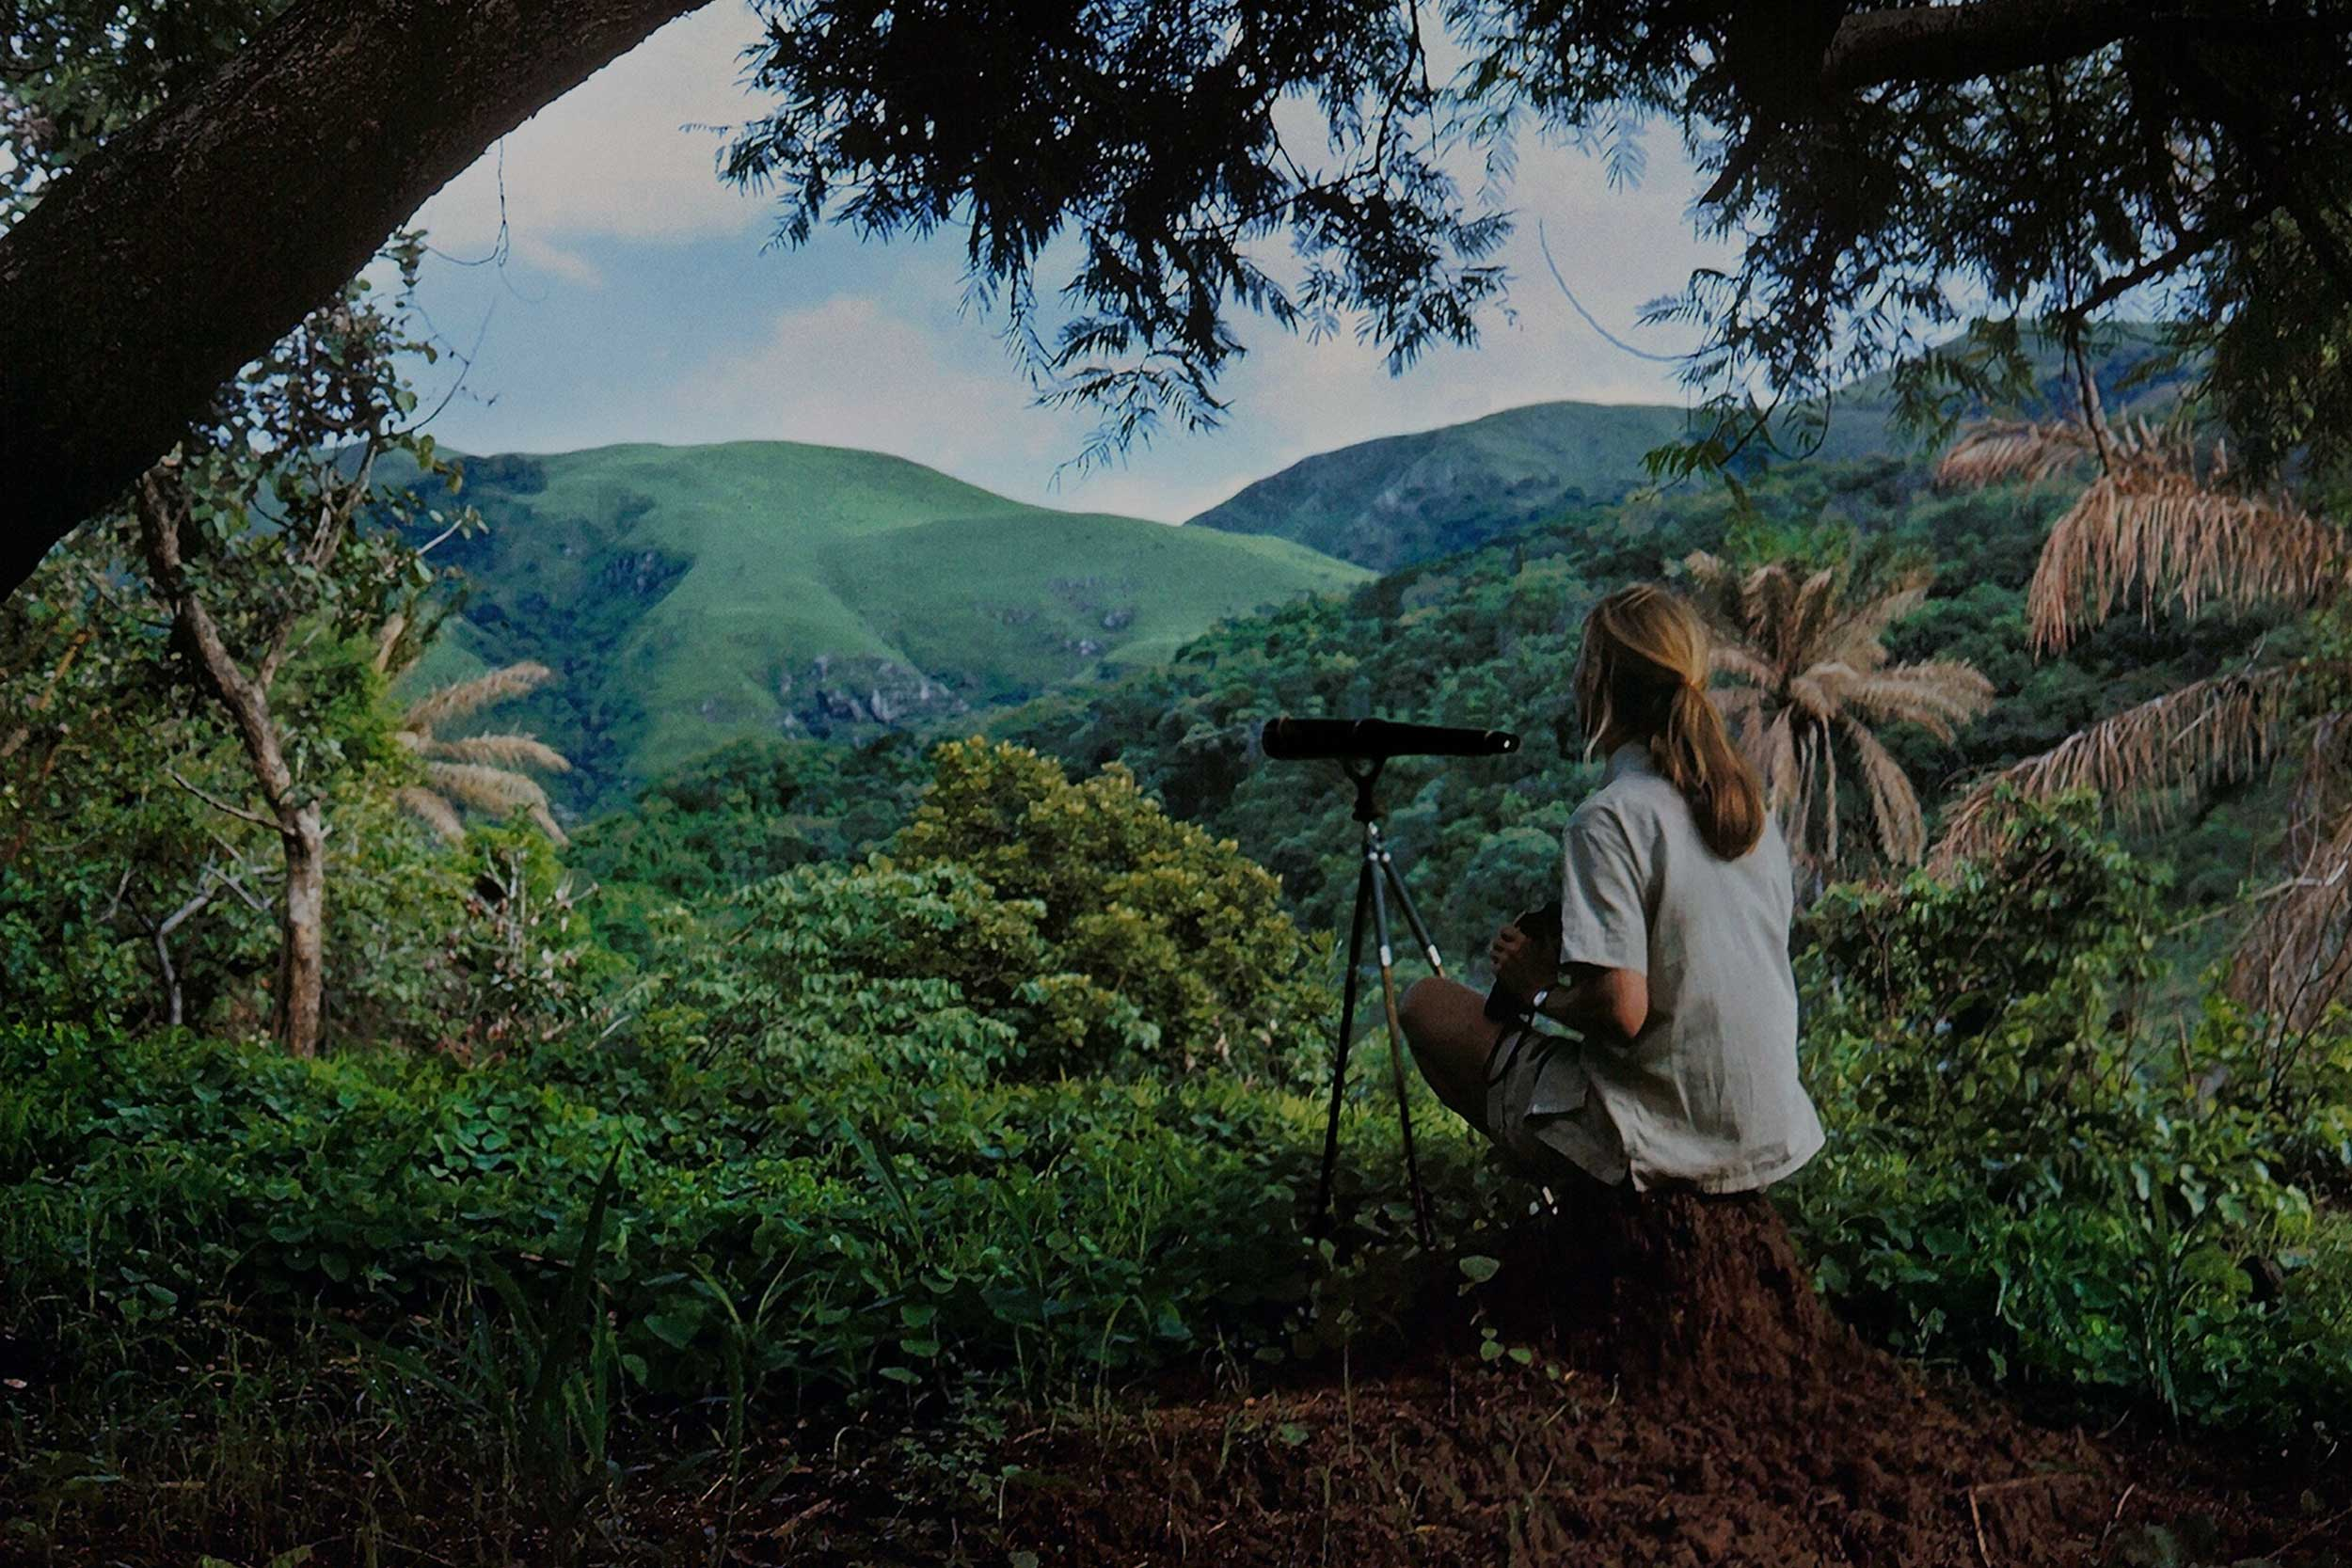
\includegraphics[
    width=8cm,
    height=8cm,
    keepaspectratio
]{jane-goodall-forest}

Goodall did this with the objective of helping us gain more insight into
chimpanzees and their relation with humans.

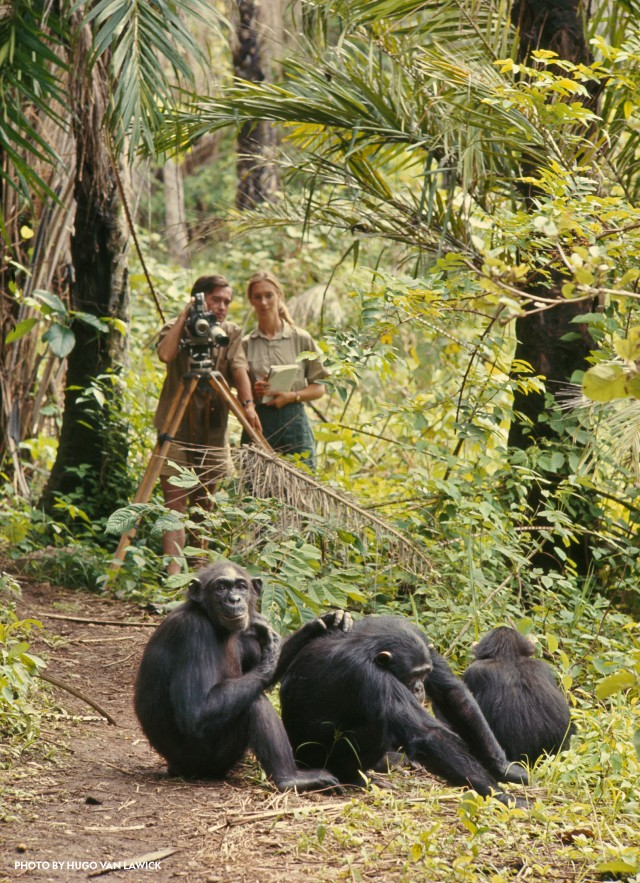
\includegraphics[
    width=10cm,
    height=10cm,
    keepaspectratio
]{jane-goodall-observing-2}

\pagebreak

And 5 years later, leading us to 1965, Jane Goodall finally earned her Ph.D.
from Cambridge University for her groundbreaking research on wild chimpanzees.

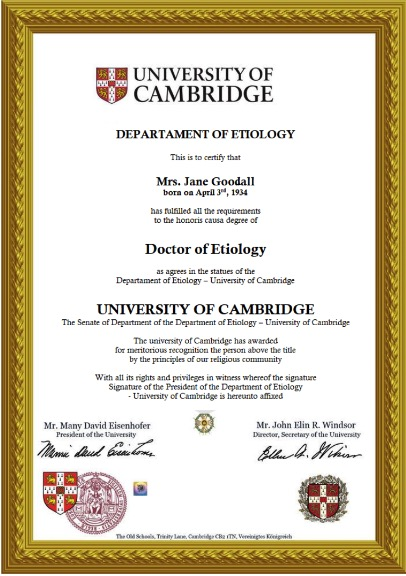
\includegraphics[
    width=10cm,
    height=10cm,
    keepaspectratio
]{jane-goodall-phd}

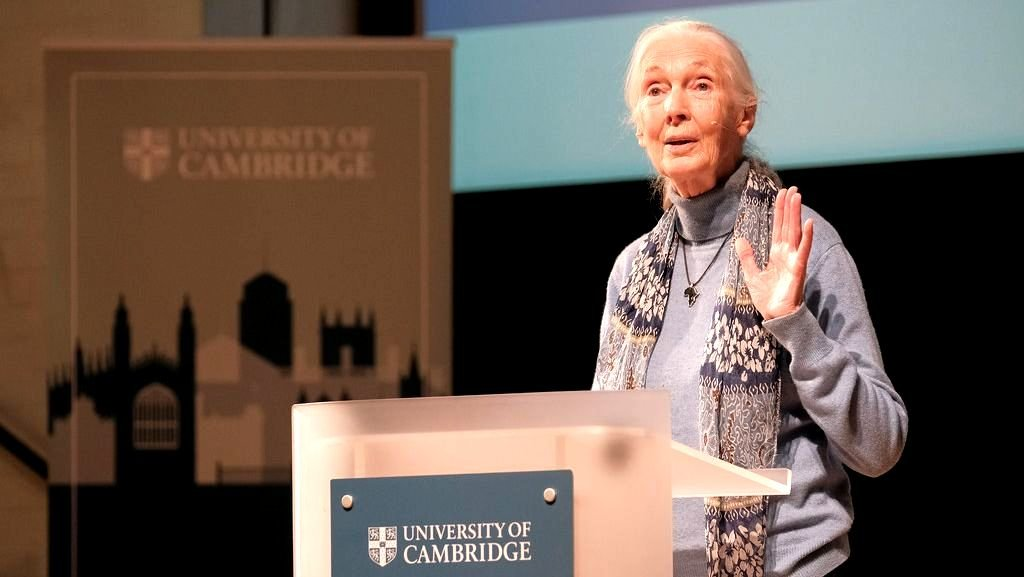
\includegraphics[
    width=11cm,
    height=11cm,
    keepaspectratio
]{jane-goodall-university-speech}

\pagebreak

This is around the time when Goodall was married to Derek Bryceson in 1975,
adding on the excitement Goodall had after just receiving her Ph.D.

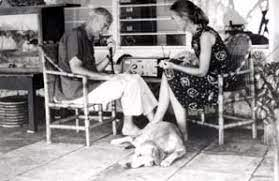
\includegraphics[
    width=9cm,
    height=9cm,
    keepaspectratio
]{jane-goodall-bryceson-3}

Interestingly, Bryceson served as a director of the Tanzanian Park System, and
a former director of a park. Just before his marriage, he was also the minister
for Agriculture and Cooperatives.

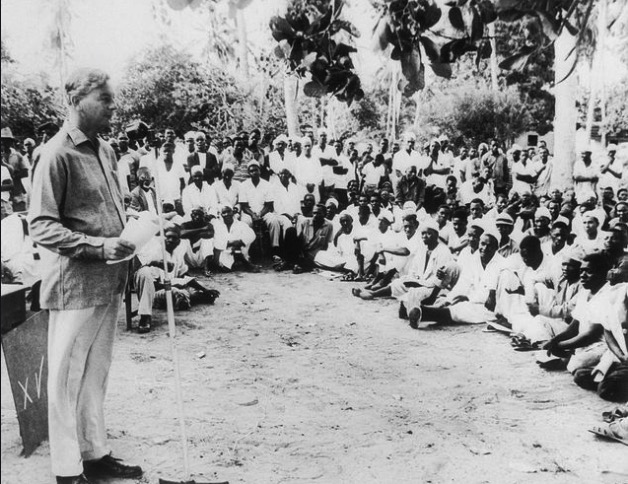
\includegraphics[
    width=9cm,
    height=9cm,
    keepaspectratio
]{bryceson}

\pagebreak

But sadly, that marriage only lasted for 5 years. Goodall was alone.

"He got this horrible cancer. That was the end."

"I didn't meet the right person, I suppose, or potentially the right person."

Goodall hasn't seen much point in pursuing love again, the end result is always
the same. Instead she has continued her work moving forward.

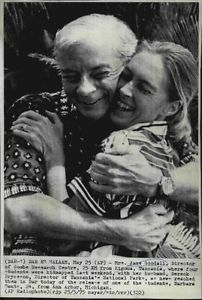
\includegraphics[
    width=11cm,
    height=11cm,
    keepaspectratio
]{jane-goodall-bryceson-2}

\pagebreak


\includegraphics[
    width=11cm,
    height=11cm,
    keepaspectratio
]{jane-goodall-institute}

2 years later, Goodall found the courage after the death of her husband to
start the Jane Goodall Institute, to preserve African apes alongside their
habitats.

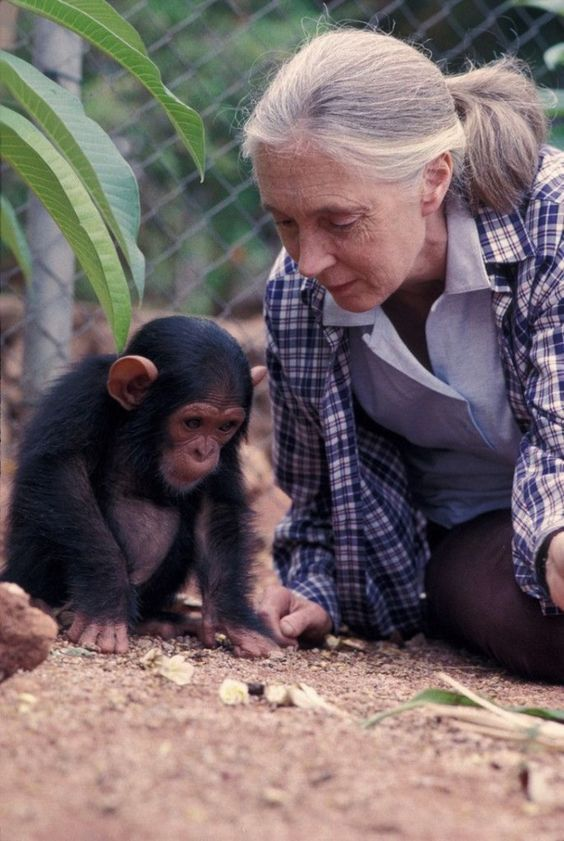
\includegraphics[
    width=9cm,
    height=9cm,
    keepaspectratio
]{jane-goodall-baby-chimp}

As what we've seen from Goodall's research, this institute will mainly focus on
chimpanzees.

\pagebreak

And 9 years later, all the hard work that had been put in Goodall's research
back in Gombe 26 years ago, has resulted in a book---\textit{"The Chimpanzees
of Gombe: Patterns of Behavior"}.

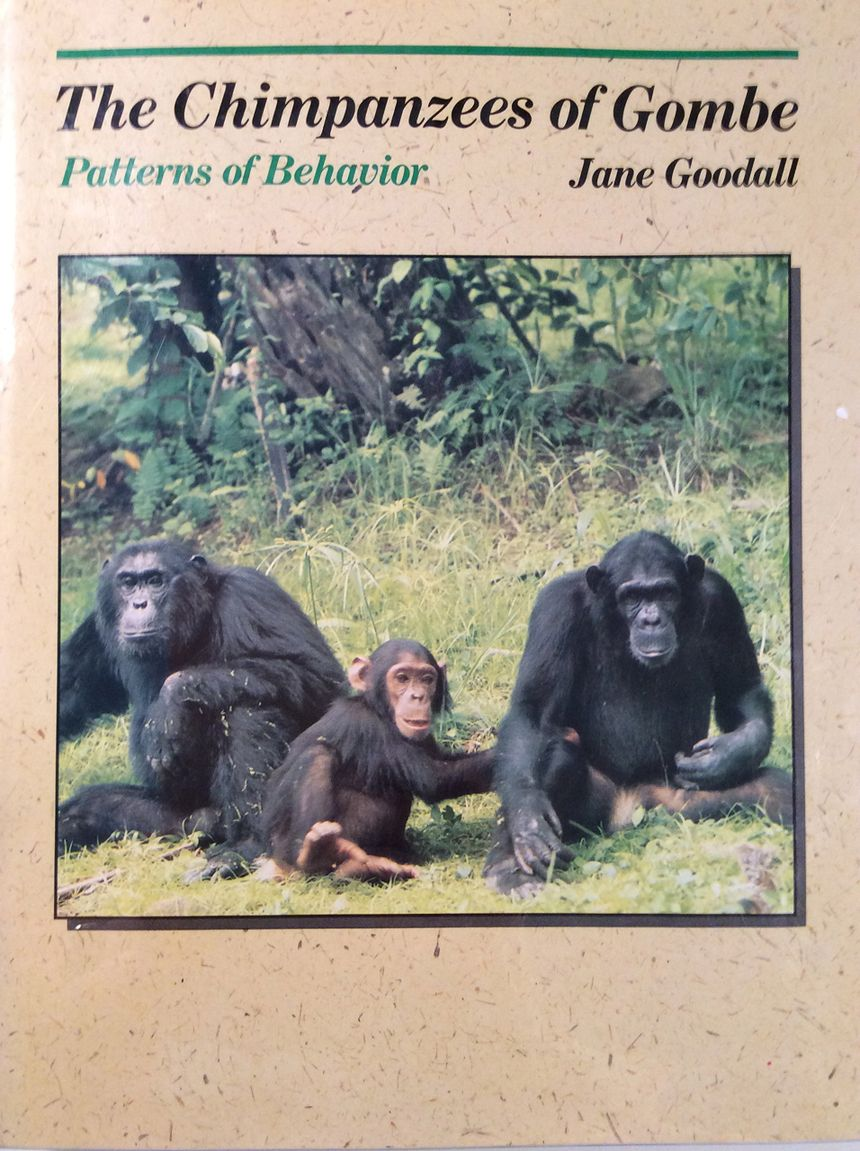
\includegraphics[
    width=13cm,
    height=13cm,
    keepaspectratio
]{the-chimps-of-gombe}

This book perfectly sums up two decades and a half of research, explaining what
separates the chimpanzees from Gombe with other chimps.

\pagebreak

\section*{What Next?}

In 2002, after 16 years, Goodall is appointed to serve as the United Nation's
Messenger of Peace, raising awareness of the UN's efforts in improving the
lives of billions of people across the globe.

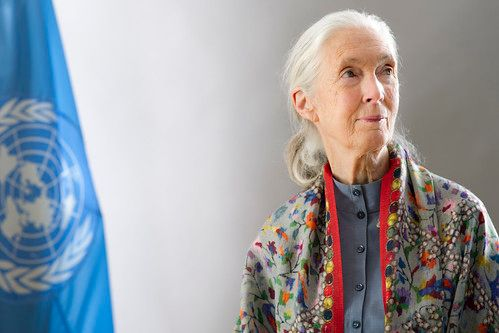
\includegraphics[
    width=10cm,
    height=10cm,
    keepaspectratio
]{jane-goodall-un-messenger}

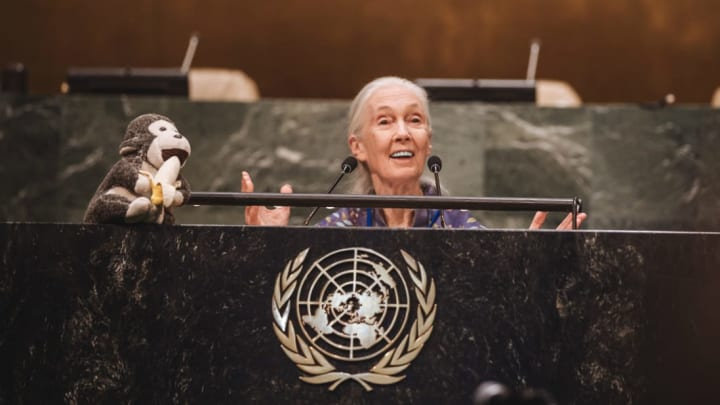
\includegraphics[
    width=13cm,
    height=13cm,
    keepaspectratio
]{jane-goodall-un-messenger-2}

\pagebreak

Adding the number of Goodall's roles, she was also knited as the Dame of the
British Empire just one year later in 2004 for her work and dedication.

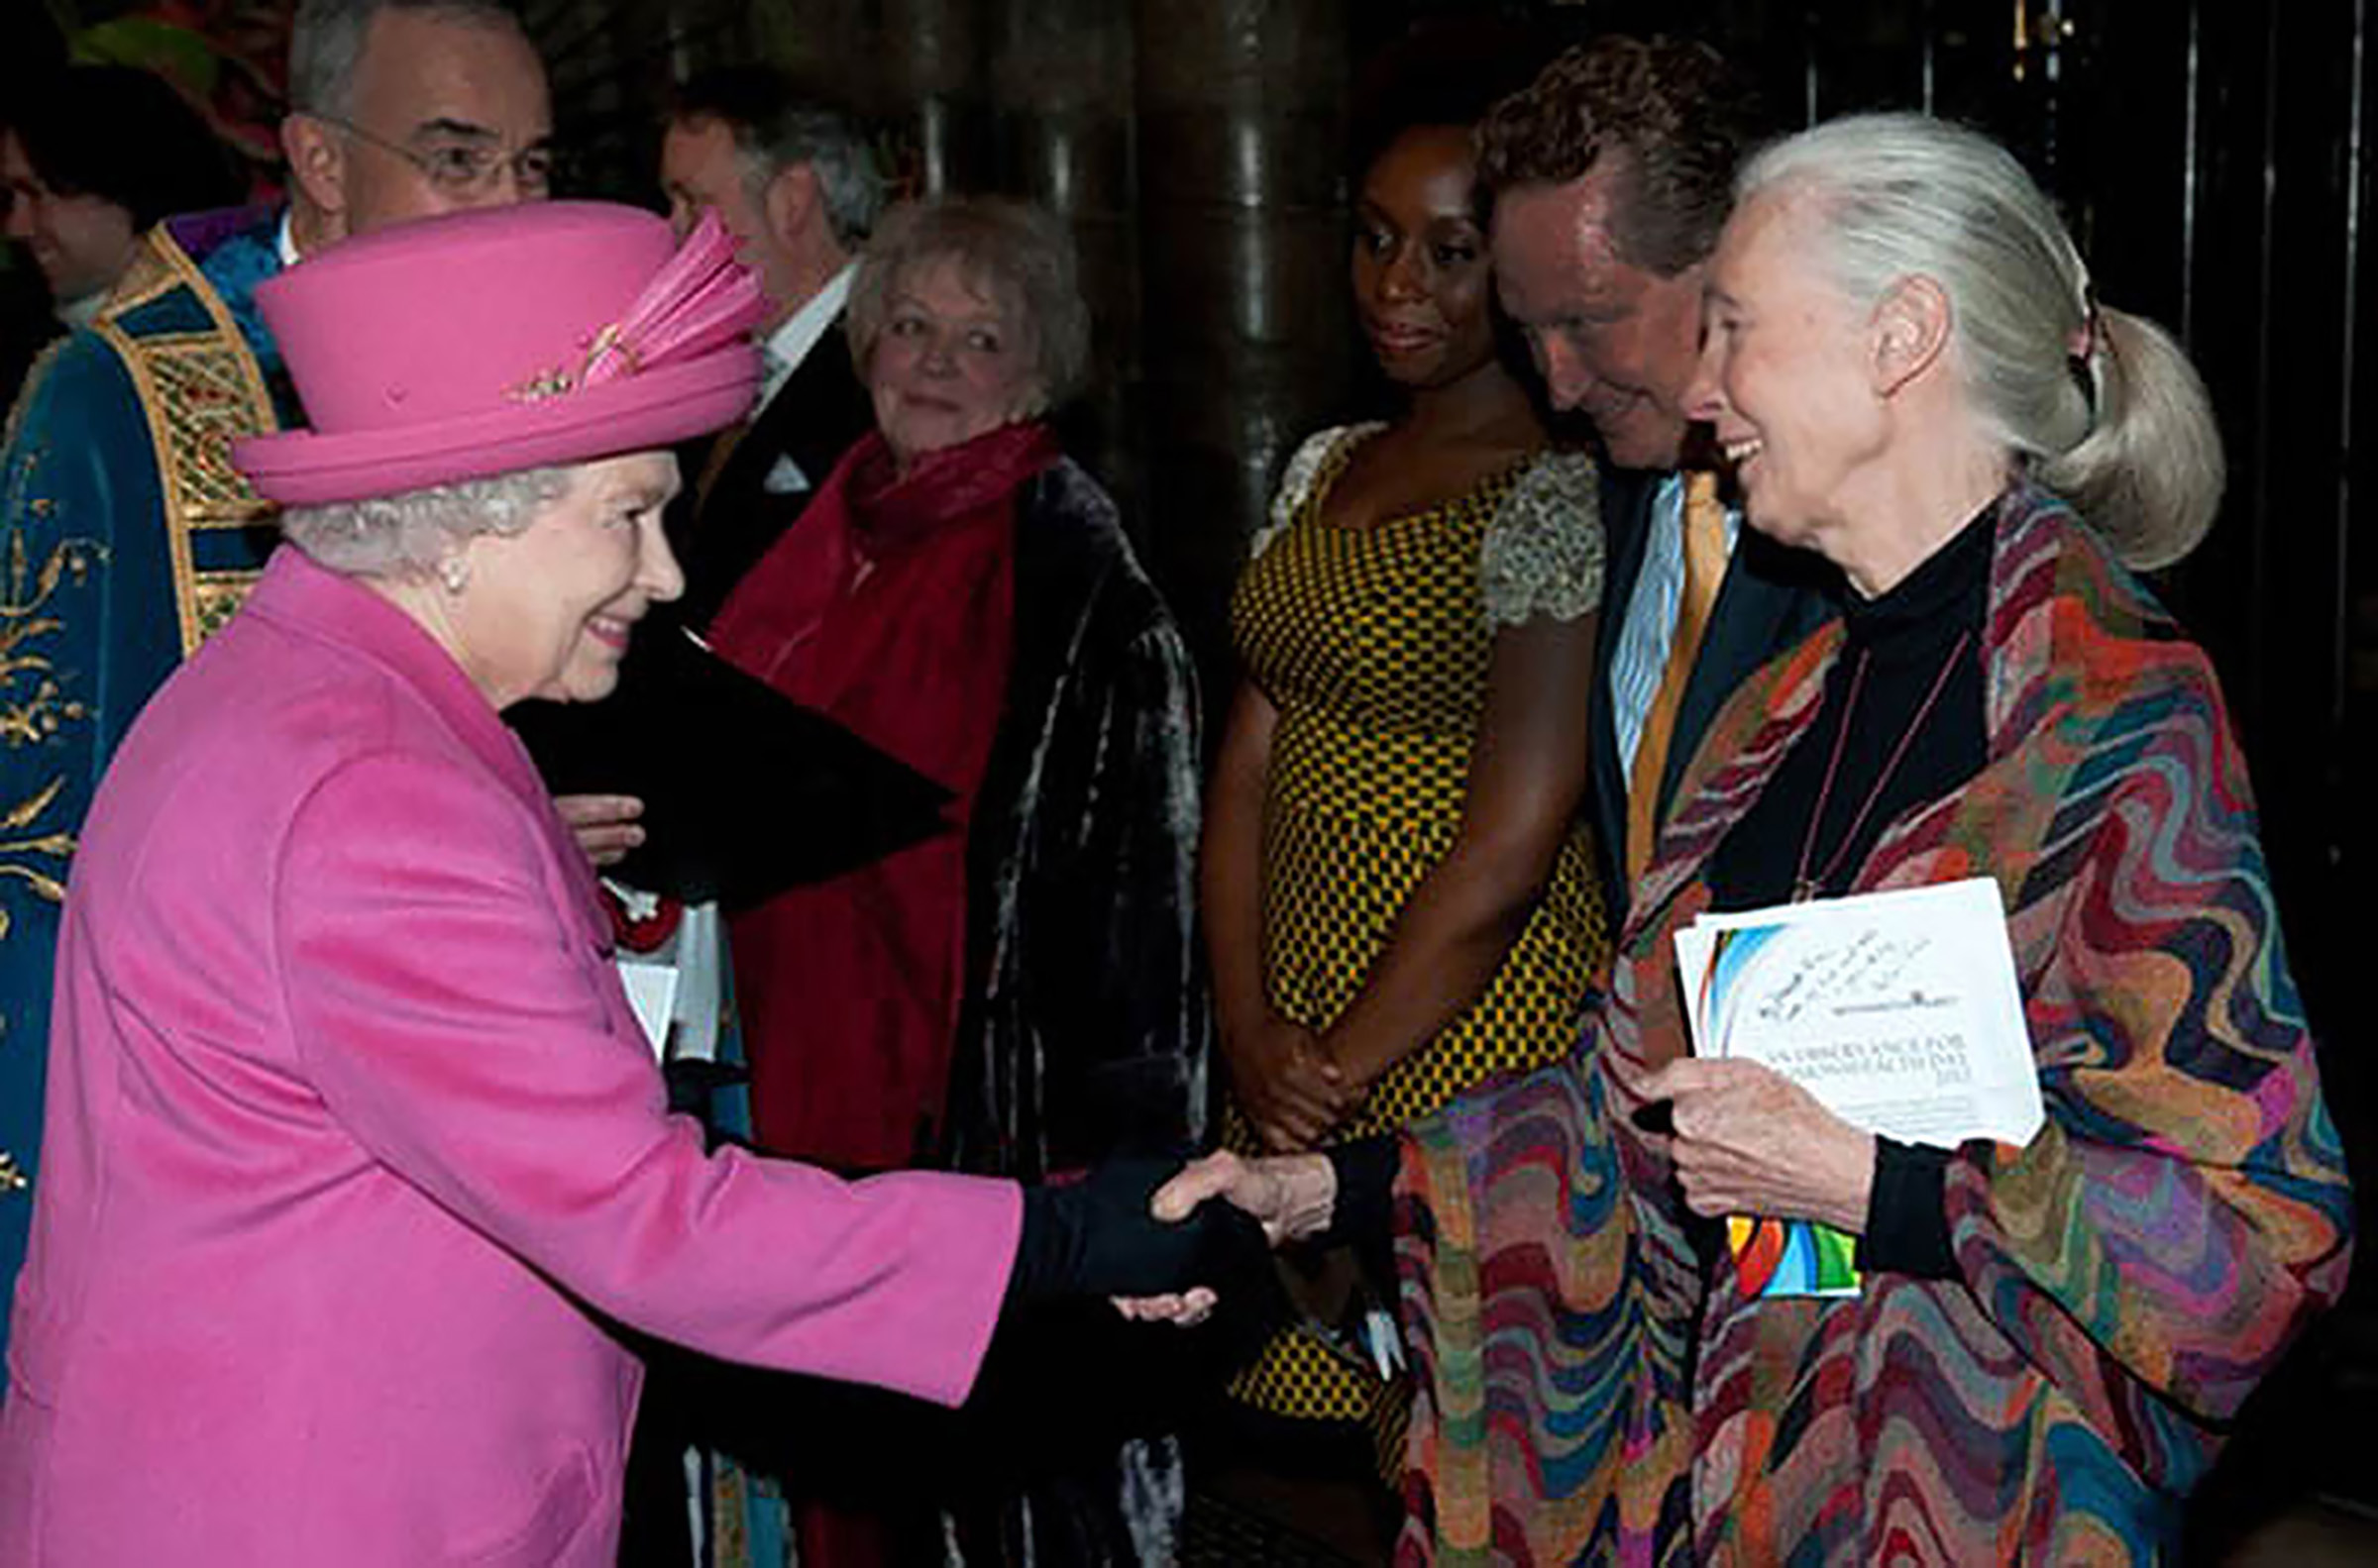
\includegraphics[
    width=13cm,
    height=13cm,
    keepaspectratio
]{jane-goodall-dame}

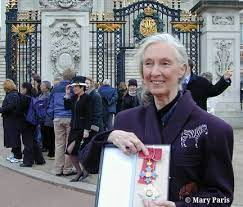
\includegraphics[
    width=10cm,
    height=10cm,
    keepaspectratio
]{jane-goodall-dame-2}

\pagebreak

Goodall also received the Discovery and Imagination Award in 2005 before
acquiring a Tyler prize for Environmental Achievement 16 years later in 2021.

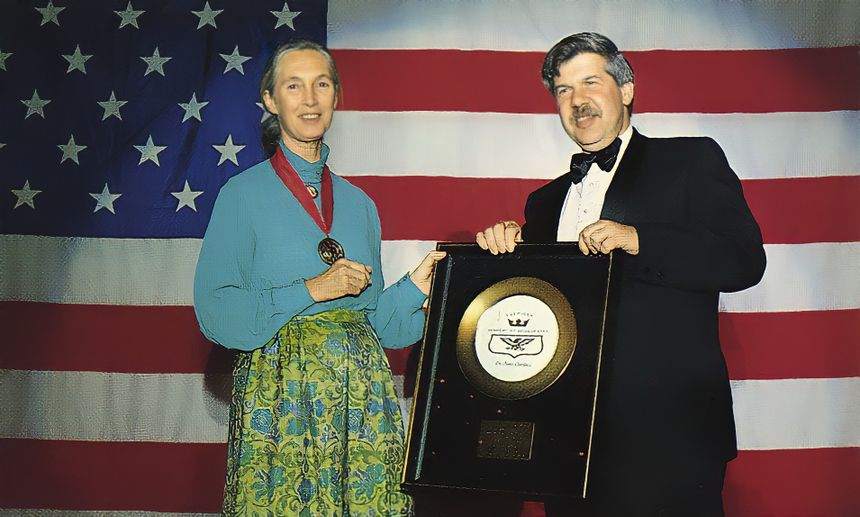
\includegraphics[
    width=10cm,
    height=10cm,
    keepaspectratio
]{jane-goodall-award}

During this period, Goodall started making more books to spread hope and
awareness surrounding chimpanzees and even the environment.

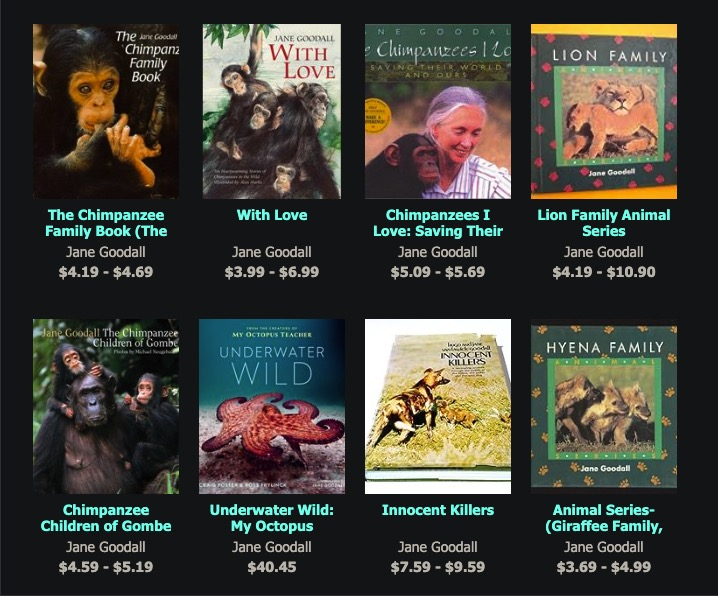
\includegraphics[
    width=10cm,
    height=10cm,
    keepaspectratio
]{jane-goodall-books}

\pagebreak

In 2021, Goodall gave an inspiring speech when she received the Stephen Hawking
medal, a highly-acclaimed award on an international level from the Starmus
Festival.

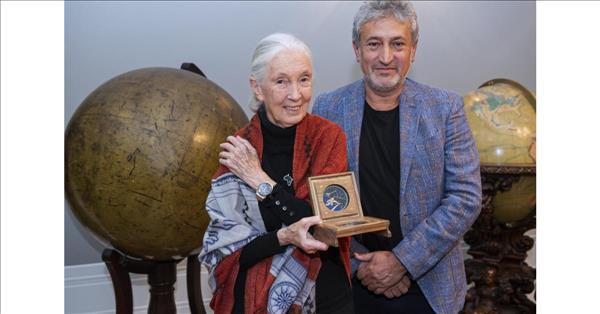
\includegraphics[
    width=10cm,
    height=10cm,
    keepaspectratio
]{jane-goodall-hawking-medal}

This medal is intended for individuals who have conveyed complex scienctific
concepts to the general public, therefore advocating a better understanding of
science in general.

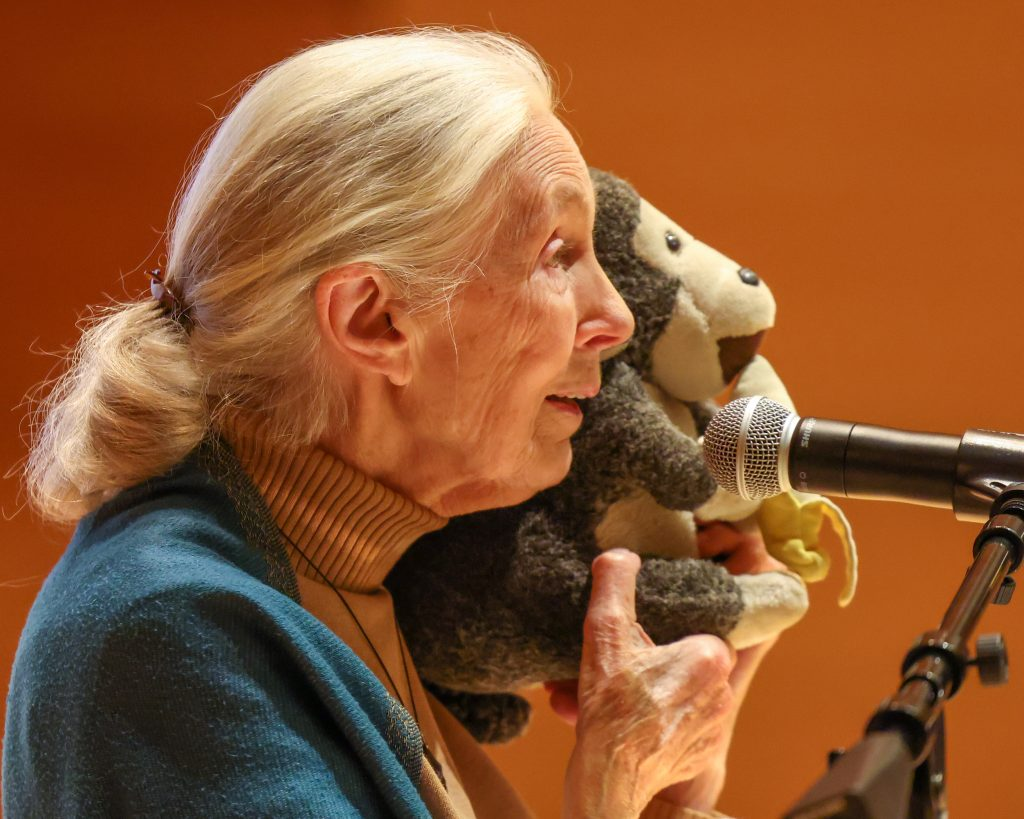
\includegraphics[
    width=10cm,
    height=10cm,
    keepaspectratio
]{jane-goodall-speech}

\pagebreak

And just a year later, in 2022, due to Goodall achieveing the level of success
she did over the past 40 years, she was even made into the \textit{LEGO} set
\textit{"Jane Goodall Tribute"}.

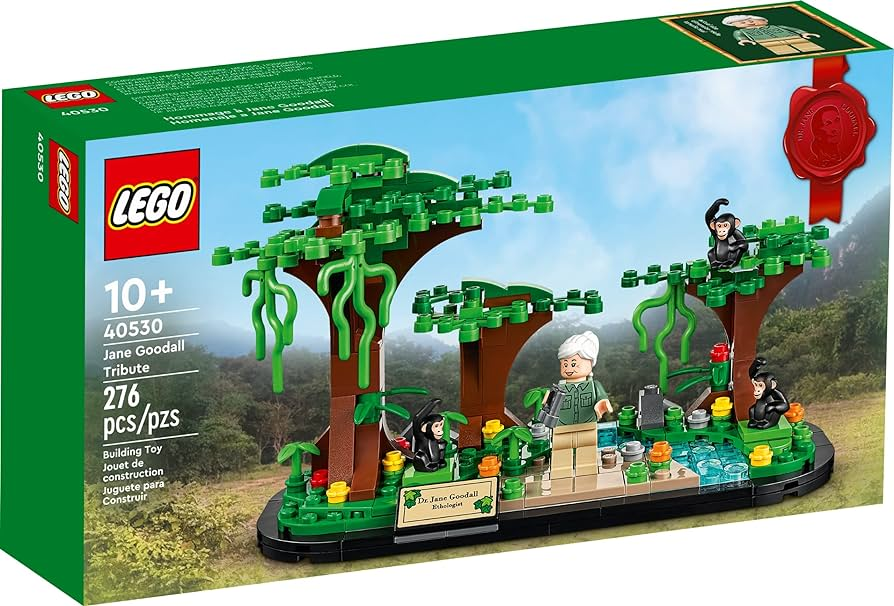
\includegraphics[
    width=10cm,
    height=10cm,
    keepaspectratio
]{jane-goodall-lego}

Someone nicknamed \textit{MrEvilDuck} even stepped in and made a modification
to the set, expanding the overall size. They then posted it in \textit{r/lego}
and received 1300 upvotes.

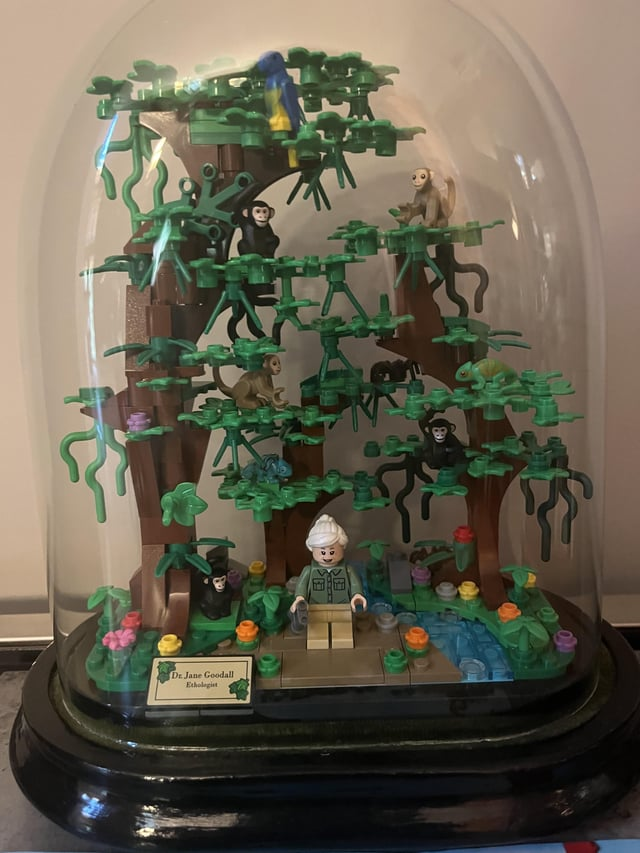
\includegraphics[
    width=7cm,
    height=7cm,
    keepaspectratio
]{jane-goodall-lego-modified}

\pagebreak

Even to this day, Dr. Jane Goodall continues to travel around the world,
spreading hope through writing, speaking, and most importantly, action.

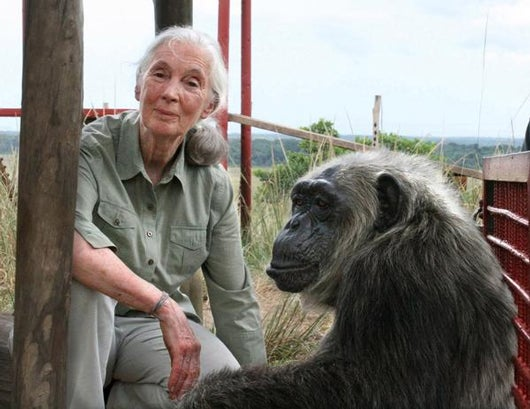
\includegraphics[
    width=10cm,
    height=10cm,
    keepaspectratio
]{jane-goodall-old}

“I do have reasons for hope: our clever brains, the resilience of nature, the
indomitable human spirit, and above all, the commitment of young people when
they’re empowered to take action.”

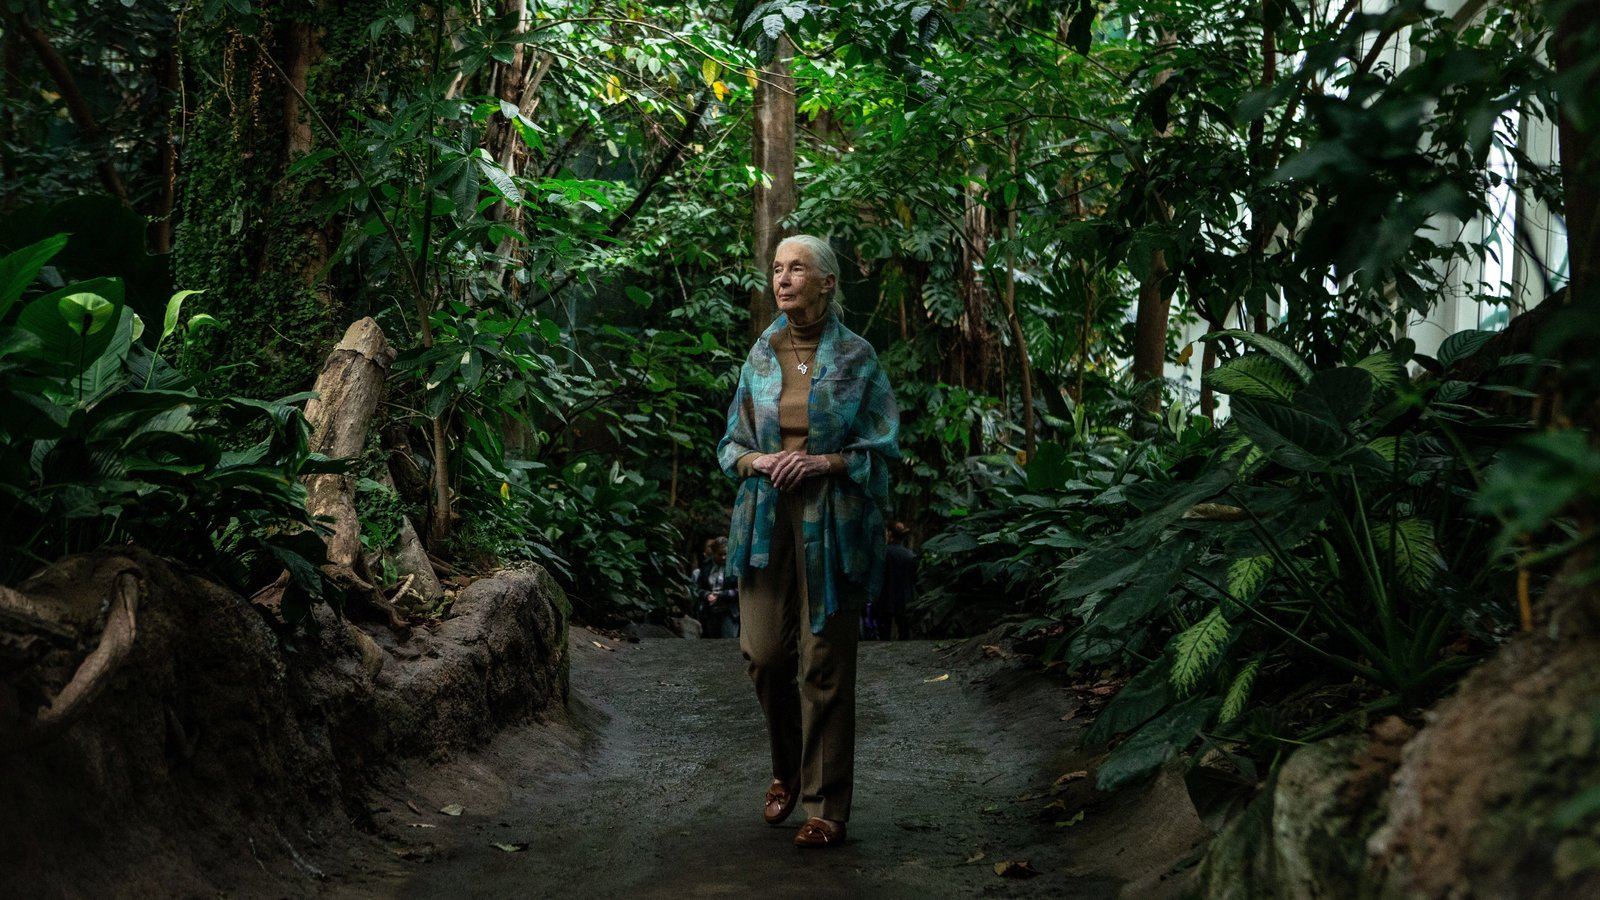
\includegraphics[
    width=13cm,
    height=13cm,
    keepaspectratio
]{jane-goodall-ending-note}

\end{document}
